\hypertarget{cv:gestionarBR}{\section{Gestionar Reglas de Negocio}} \label{sec:GestionarBR}

	Esta funcionalidad le permitirá las acciones necesarias para controlar las regla de negocio y visualizarlos en una tabla en el proyecto sobre el que se está operando y solicitar el registro de uno nueva.

		\subsection{Procedimiento}

			%Pasos de procedimiento
			\begin{enumerate}
				
			\item Ingrese a un proyecto existente desde la pantalla \ref{fig:GestionarProyectosColaborador}.
	
			\item Seleccione la opción \textbf{Reglas de negocio} del menú \ref{fig:MN-LPC}.
	
			\item Se mostrará la pantalla \ref{fig:GestionarBR} ''Gestionar Reglas de negocio''.

			%Pantalla
			\begin{figure}[h!]
				\begin{center}
					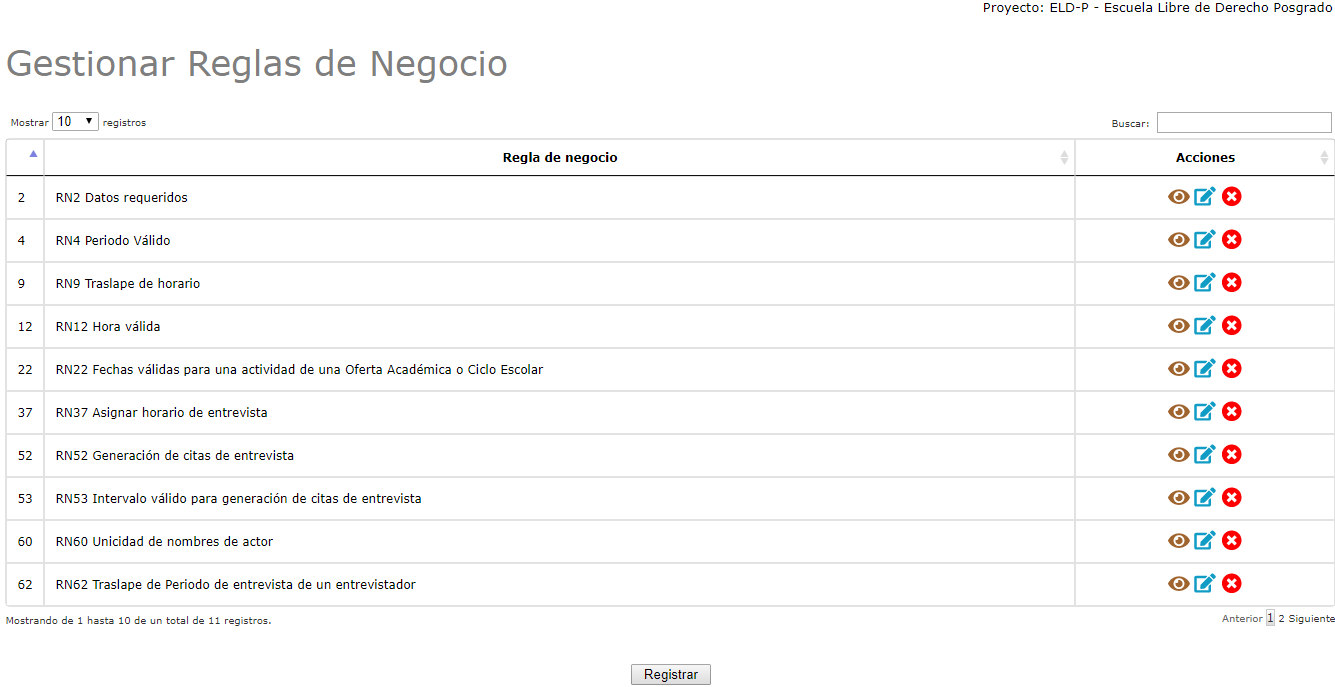
\includegraphics[scale=0.5]{roles/lider/reglasNegocio/pantallas/IU8gestionarBR}
					\caption{Gestionar Reglas de Negocio}
					\label{fig:GestionarBR}
				\end{center}
			\end{figure}
		
				\item Seleccione la operación que desea realizar:
			
			Para (\hyperlink{cv:registrarBR}{Registrar}) dé clic en el botón \IURegistrar.
			
			Para (\hyperlink{cv:modificarBR}{Modificar}) dé clic en el icono \IUEditar{} de alguna regla de negocio ya registrada.
			
			Para (\hyperlink{cv:eliminarBR}{Eliminar}) dé clic en el icono \IUBotonEliminar{} de alguna regla de negocio ya registrada.
			
			Para (\hyperlink{cv:consultarBR}{Consultar}) dé clic en el icono \IUConsultar{} de alguna regla de negocio ya registrada.
			\end{enumerate}